	\documentclass[11pt, a4paper, spanish]{article}

\usepackage{alltt}

%%%%%%%%%% COMIENZO DEL PREAMBULO %%%%%%%%%%

%Info sobre este documento
\author{Mart\'n Cammi}
\title{Trabajo Pr\'actico de Algoritmos y Estucturas de datos III}

%\usepackage{infostyle}                                                  % provee un look & feel similar a un documento Word
\usepackage[top=2.5cm, bottom=2.5cm, left=2.5cm, right=2.5cm]{geometry}  % m\'argenes
\usepackage[ansinew]{inputenc}                                           % permite que los acentos del estilo \'a\'e\'i\'o\'u salgan joya
\usepackage[spanish, activeacute]{babel}                                 % idioma espaniol, acentos f\'aciles y deletreo de palabras
\usepackage{indentfirst}                                                 % permite indentar un parrafo a mano
\usepackage{caratula}                                                    % incluye caratula est\'andar
\usepackage{graphicx}                                                    % permite insertar gr\'aficos
\usepackage{color}                                                       % permite el uso de colores en el documento
\usepackage{amssymb}
\usepackage[pdfcreator={TexLive!, LaTeX2e con TeXnicCenter},
			pdfauthor={Grupo: "1"},
			pdftitle={Algoritmos III - Trabajo Pr\'actico 2},
			pdfsubject={Trabajo Pr\'actico 1},
			pdfkeywords={Prismas, Esferas, Punto de corte, puente, pizza},
			pdfstartview=FitH,            % Fits the width of the page to the window
			bookmarksnumbered,            % los bookmarks numerados se ven mejor...
			colorlinks,                   % links con bellos colores
			linkcolor=magenta]            % permite cambiar el color de los links
			{hyperref}                    % Permite jugar con algunas cosas que aparecer\'an en el PDF final

%RESTAURAR

\usepackage{algorithm}							% Permite tabular un codigo
\usepackage{algorithmic}
%\floatname{algorithm}{Algoritmo}
\renewcommand{\listalgorithmname}{Lista de algoritmos}
\renewcommand{\algorithmicrequire}{\textbf{Entrada:}}
\renewcommand{\algorithmicensure}{\textbf{Salida:}}
\renewcommand{\algorithmicend}{\textbf{fin}}
\renewcommand{\algorithmicif}{\textbf{si}}
\renewcommand{\algorithmicthen}{\textbf{entonces}}
\renewcommand{\algorithmicelse}{\textbf{si no}}
\renewcommand{\algorithmicelsif}{\algorithmicelse,\ \algorithmicif}
\renewcommand{\algorithmicendif}{\algorithmicend\ \algorithmicif}
\renewcommand{\algorithmicfor}{\textbf{para}}
\renewcommand{\algorithmicforall}{\textbf{para todo}}
\renewcommand{\algorithmicdo}{\textbf{hacer}}
\renewcommand{\algorithmicendfor}{\algorithmicend\ \algorithmicfor}
\renewcommand{\algorithmicwhile}{\textbf{mientras}}
\renewcommand{\algorithmicendwhile}{\algorithmicend\ \algorithmicwhile}
\renewcommand{\algorithmicloop}{\textbf{repetir}}
\renewcommand{\algorithmicendloop}{\algorithmicend\ \algorithmicloop}
\renewcommand{\algorithmicrepeat}{\textbf{repetir}}
\renewcommand{\algorithmicuntil}{\textbf{hasta que}}
\renewcommand{\algorithmicprint}{\textbf{imprimir}} 
\renewcommand{\algorithmicreturn}{\textbf{devolver}} 
\renewcommand{\algorithmictrue}{\textbf{cierto }} 
\renewcommand{\algorithmicfalse}{\textbf{falso }} 
 % mi archivo de traducci\'on			

%\selectlanguage{spanish}

%\selectlanguage{spanish}
\linespread{1.3}                    % interlineado equivalente al 1.5 l\'ineas de Word...
\pagestyle{myheadings}              %encabezado personalizable con \markboth{}{}
\markboth{}{Algoritmos III  - Trabajo Pr\'actico 3 - Cammi, Garbi, Kretschmayer}
\headsep = 30pt                     % separaci\'on entre encabezado y comienzo del p\'arrafo

%\addtolength{\oddsidemargin}{-2cm}	% configuracion IDEAL!!!
%\addtolength{\textwidth}{4cm}
%\addtolength{\textheight}{2cm}

% macro 'todo' para To-Do's
\def\todo#1{\textcolor{red}{#1}}

% Macro 'borde' para un texto con borde
\newsavebox{\fmbox}
\newenvironment{borde}[1]
{\begin{lrbox}{\fmbox}\begin{minipage}{#1}}
{\end{minipage}\end{lrbox}\fbox{\usebox{\fmbox}}\\[10pt]}

%%%%%%%%%% FIN DEL PREAMBULO %%%%%%%%%%

\begin{document}

\materia{Algoritmos y Estucturas de datos III}
\submateria{Segundo Cuatrimestre de 2011}
\titulo{Trabajo Pr\'actico 3}
\subtitulo{Cartero Chino en grafo mixto.}
\grupo{Grupo: `1'}
\integrante{Cammi, Mart\'in}{676/02}{martincammi@gmail.com}
\integrante{Garbi, Sebasti\'an}{179/05}{garbyseba@gmail.com}
\integrante{Kretschmayer, Daniel}{310/99}{daniak@gmail.com}

\maketitle

\thispagestyle{empty}

\tableofcontents

\newpage


\textbf{Ejecuci\'on del TP}
\label{sec:ejecucion}

	\subsection{Lenguaje utilizado}
		
		El lenguaje utilizado para el trabajo pr\'actico ha sido \emph{Java}, compilando con la versi\'on 1.5 de la Virtual Machine.
		
		El trabajo se acompa\~{n}a con los fuentes de la soluci\'on que puede importarse en IDE de Eclipse o ejecutarse desde l\'inea de comandos.

	\subsection{Como ejecutar el TP}
	
	\textbf{\underline{Desde l\'inea de comandos}}
	\begin{itemize}
			\item{Posicionarse en el directorio Algo3Tp3}
			\item{Copiar all\'i el archivo de entrada para el problema i, por ejemplo Ej1.in}
			\item{Ejecutar el comando: \emph{java -cp ./bin problema1.Ej1}}
	\end{itemize}
	Esto generar\'a el archivo Ej1.out con la soluci\'on en el mismo directorio Algo3Tp3.

	\textbf{\underline{Desde el Eclipse}}
	
	Primero importaremos el proyecto:	
	
	\begin{itemize}
			\item{Seleccionar File $\Rightarrow$ Import.}
			\item{Seleccionar General $\Rightarrow$ Existing Projects into Workspace $\Rightarrow$ Next.}
			\item{Seleccionar el directorio llamado Algo3Tp3.}
			\item{Finish.}
	\end{itemize}
	
	Desde la vista de \textbf{Package Explorer} bajo el paquete \textbf{src} aparecer\'an tres paquetes m�s y dentro de cada uno de ellos los siguientes archivos de java:\\

	\begin{center}
		%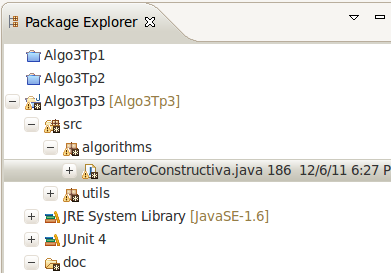
\includegraphics[scale=0.65]{others/packageExplorer.png}\\
		COLOCAR IMAGEN CORRECTA
	\end{center}

\newpage

	Para ejecutar un problema:

	\begin{itemize}
			\item{Posicionarse en el directorio Algo3Tp3}
			\item{Copiar en el directorio Algo3Tp3 el archivo de entrada para el problema i, por ejemplo Ej1.in}
			\item{Con bot\'on derecho Run As $\Rightarrow$ Java Application. Se ejecutar\'a el problema seleccionado.}
	\end{itemize}
	Esto generar\'a el archivo Ej1.out con la soluci\'on en el mismo directorio Algo3Tp3.

\newpage


\section{Introducci\'on}

	En 1736 Leonhard Euler public\'o un trabajo en el cual resolv\'ia el denominado \emph{problema de los puentes de K\"{o}nigsberg}. La ciudad de K\"{o}ningsberg, actual Kaliningrado, Rusia, est� dividida por el r\'io Pregel en 4 zonas, dos orillas (A y B), la isla de Kneiphof (C) y otras dos partes divididas por el r�o. (D y F). Las orillas estaban conectadas mediante 7 puentes. El problema consist�a partir de una orilla y recorrer todos los puentes, recorri\'endo una sola vez cada uno y volviendo al punto de partida.\\

Este fu\'e el puntapi� inicial para un tipo de problema que m'as adelante de modelar\'ia usando la teor\'ia de grafos. Este problema fue caracterizado por Euler y consist\'ia en encontrar un circuito que pasara por todas las aristas de un grafo una s\'ola vez volviendo al punto de partida.\\
 
M\'as de doscientos a\~{n}os m\'as tarde en 1962 el matem�tico chino Kwan Mei-Koo public� un paper en el que abordaba un problema ligeramente similar, propon\'ia que si un grafo no pose\'ia un circuito Euleriano, podria quiz�s encontrar el circuito m\'as corto que pasara por todas las aristas aunque repitiera algunas de ellas. Este problema fue luego nombrado como "Problema del cartero chino".

\begin{center}
\centering 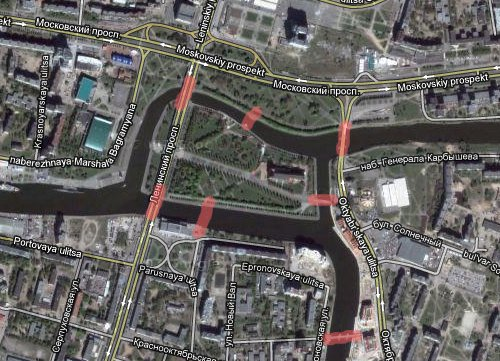
\includegraphics[scale=0.70]{img/KaliningradoBridges.jpg}\\
\small{Imagen actual de la ciudad de Kaliningrado, en rojo figuran los puentes del problema original de K\"{o}nigsberg algunos cuales ya no existen hoy en d\'ia.}
\end{center}	

El problema tiene varias variantes, en este trabajo abordaremos la variante \emph{mixta} que consiste en intentar encontrar el m\'inimo circuito que pase por todas las aristas (no orientadas) y arcos (orientadas) de un grafo donde cada una tiene peso asignado.

\section{Situaciones de la vida real}

    El algoritmo del cartero chino tiene m�ltiples aplicaciones en la vida cotidiana por ser

	\begin{itemize}
	\item C\'alculo de rutas \'optimas para recorridos de camiones de basura: en donde los camiones deban recorrer las calles de una ciudad y volver al centro de tratamiento de basura. Las calles podr\'ian bien tener diferentes sentidos o sentidos �nicos, y los pesos podr\'an corresponder a la cantidad de basura que deban recolectar en ciertas zonas.
	\end{itemize}


\section{Heur�stica Constructiva}
	Para la etapa constructiva, hemos realizado en primer lugar, una orientaci\'on de todas las aristas utilizando 5 maneras distintas, todas ellas con respecto a los grados de los nodos. Entonces, seg\'un un par\'ametro de entrada que indica cual de estas opciones usar\'a, encontrar\'a los nodos del grafo que cumplan lo siguiente, pas\'andole otro par\'ametro y buscar\'a: 
	
	\begin{itemize}
	
	\item Los nodos que tienen igual cantidad de aristas sin orientar que orientadas, y en caso de haber muchos, solo tomar\'a los primeros k nodos de ellos, donde k es el par\'ametro de entrada de la funci\'on.
	\item Los nodos a partir de un cierto n\'umero, que es definido por el par\'ametro de entrada de la funci\'on.
	\item Los nodos que tengan grado de nodo (sin orientar) mayor o igual al par\'ametro de entrada de la funci\'on.
	\item Los nodos que tengan grado de entrada (orientado) mayor o igual al par\'ametro de entrada de la funci\'on.
	\item Los nodos que tengan grado de salida (orientado) mayor o igual al par\'ametro de entrada de la funci\'on.
 
  \end{itemize}
  
  En caso de no encontrar ning\'un nodo a orientar con estas opciones, encontr\'a los k primeros nodos (empezando desde 0), sea cual sea el grado de sus nodos.
  Con cualquiera de estas posibilidades, siempre se intenta hacer un balance entre los grados que quedar\'an (solo quedar\'an grados de entrada y salida, ya que ser\'a completamente orientado). Esta decisi�n se basa, que luego le calcularemos el circuito Euleriano al grafo resultante, para poder encontrar un circuito que pase por todas las aristas. Una vez que tenemos todo el grafo orientado, realizamos luego una etapa de matching entre los nodos que quedan con diferentes grado de entrada y de salida, y balanceamos a todos los nodos, para que queden con iguales grados de entrada como de salida, y el grafo queda Euleriano. Este matching lo calculamos con la distancia m\'inima de entre cada uno de los nodos, pero en el grafo original, por lo que todas las aristas agregadas, tienen distancia m\'inima entre ellas.
	
\section{Heur�stica de busqueda Local}
En nuestra b\'usqueda local, lo que realizaremos es cambiar el matching que hace entre los nodos, para obtener otro donde sea  m\'inimo y as\'i poder acercarnos mejor a la soluci\'on requerida. Notemos que, como los matching entre los nodos donde se ten\'ia que los grados de entrada y de salida no coincid\'ian se efect\'ua sobre el grafo original (y no con el orientado), esta es una soluci\'on \'optima para esa orientaci\'on. Luego, con el grafo totalmente orientado y Euleriano, simplemente se calcula el peso de todas las aristas, y llegamos al peso del camino requerido.\\

//DESDE ACA ES LO QUE HABIA
Nuestro algoritmo de busqueda local se basa en eliminar aristas y arcos agregados para igualar los grados de salida a los de entrada de algunos nodos y cambiarlos por un conjunto de aristas que cumplen la misma propiedad pero cuya suma es menor.
Para ello el algoritmo constructivo realiza los siguientes pasos dado un grafo mixto:

1) Orientar todas las aristas no orientadas del grafo.
2) Calcular un matching entre los nodos que tengan din != dout.
3) Calcular el peso del camino m\'inimo entre los nodos del matching.

4) Calcular los caminos m\'inimos entre cada par del matching y con ellos y armar el Circuito euleriano.
//DESDE ACA ES LO QUE HABIA

\section{Metaheuristica Grasp}

%\label{sec:problema1}
%\subsection{Introducci\'on}
	

\end{document}
